% !TEX root = main.tex

\section{形态学图像处理} % Chap 9
\subsection{腐蚀与膨胀}
\begin{definition}[反射]
\[\hat{B}=\{w\mid w=-b,b\in B\}\]
\end{definition}
\begin{definition}[平移]
\[(B)_z=\{c\mid c=b+z,b\in B\}\]
\end{definition}
\begin{definition}[腐蚀]
结构元$B$可以完全含于$A$中
\[A\ominus B=\{z\mid(B)_z\subset A\}=\{z\mid(B)_z\cap A^C=\varnothing\}\]
注意最终结果只保留结构元的中心点。
腐蚀可以消除图像中的某些部分。
\end{definition}
\begin{figure}[H]
\centering
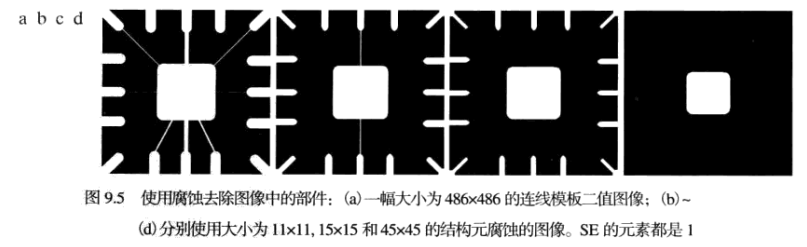
\includegraphics[width=0.9\linewidth]{fig/erosion.png}
\end{figure}
\begin{definition}[膨胀]
结构元$B$与$A$有交
\[A\oplus B=\{z\mid(\hat{B})_z\cup A\ne\varnothing\}=\{z\mid [(\hat{B})_z\cap A]\subset A\}\]
膨胀可以用来桥接裂缝。
\end{definition}
\begin{figure}[H]
\centering
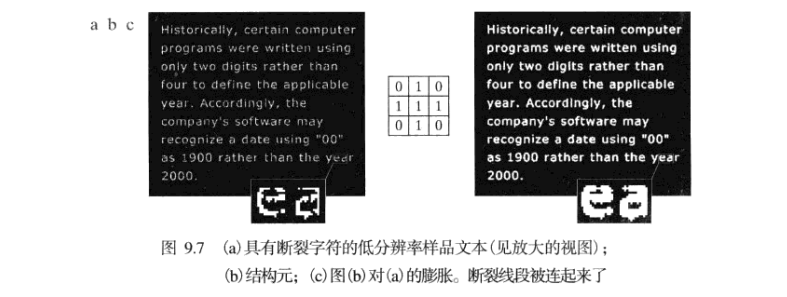
\includegraphics[width=0.9\linewidth]{fig/dilation.png}
\end{figure}

膨胀与腐蚀具有对偶性
\[\begin{aligned}
(A\ominus B)^c &= A^c\oplus B\\
(A\oplus B)^c &= A^c\ominus \hat{B}
\end{aligned}\]

\subsection{开操作与闭操作}
\begin{definition}[开操作]
$B$先对$A$腐蚀,再进行膨胀
\[A\circ B=(A\ominus B)\oplus B=\bigcup\{(B)_z\mid (B)_z\subset A\}\]
实际上就是结构元$B$在$A$内部划过的边界
\begin{figure}[H]
\centering
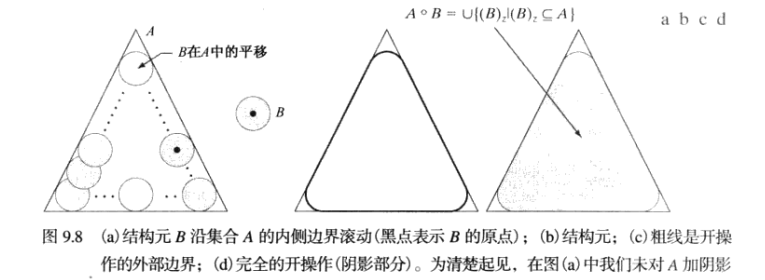
\includegraphics[width=0.9\linewidth]{fig/opening.png}
\end{figure}
\end{definition}
\begin{definition}[闭操作]
$B$先对$A$膨胀,在进行腐蚀
\[A\bullet B=(A\oplus B)\ominus B\]
实际上是结构元$B$在$A$外部划过的边界
\begin{figure}[H]
\centering
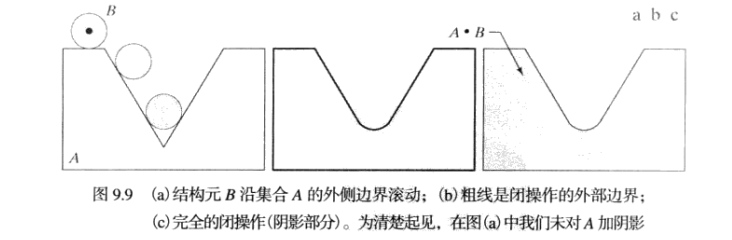
\includegraphics[width=0.9\linewidth]{fig/closing.png}
\end{figure}
\end{definition}

同样,开操作和闭操作也具有对偶性
\[\begin{aligned}
(A\bullet B)^c &= (A^c\circ\hat{B})\\
(A\circ B)^c &= (A^c\bullet\hat{B})
\end{aligned}\]

开操作和闭操作满足
\begin{itemize}
	\item $A\circ B\subset A$,$A\subset A\bullet B$
	\item 若$C\subset D$,则$C\circ B\subset D\circ B$,$C\bullet B\subset D\bullet B$
	\item $(A\circ B)\circ B=A\circ B$,$(A\bullet B)\bullet B=A\bullet B$
\end{itemize}

\subsection{击中或击不中变换}
\begin{definition}[击中或击不中(hit-or-miss)变换]
\[A\circledast B=(A\ominus D)\cap[A^C\ominus(W-D)]=(A\ominus B)\cap(A^C\ominus B_2)\]
\end{definition}
\begin{figure}[H]
\centering
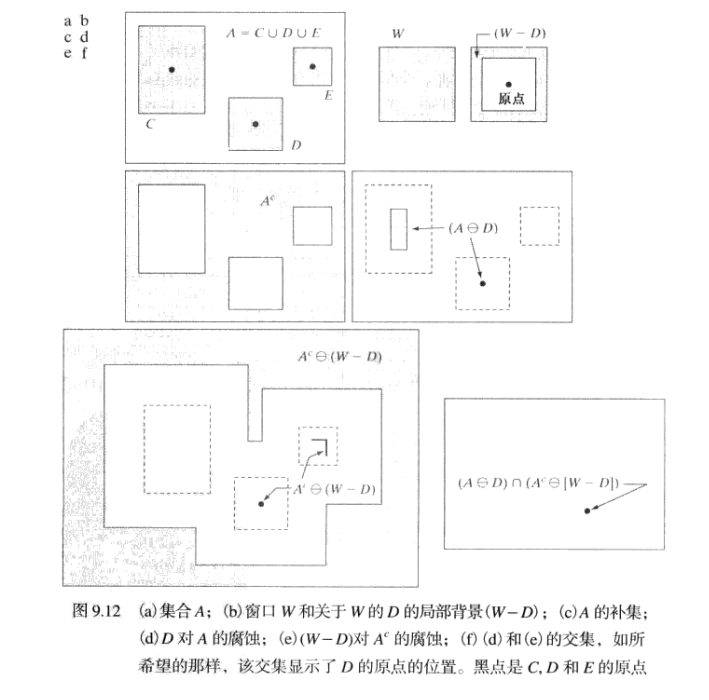
\includegraphics[width=0.9\linewidth]{fig/hit-or-miss.png}
\end{figure}

\subsection{基本形态学算法}
\begin{itemize}
\item 边界提取
\[\beta(A)=A-(A\ominus B)\]
\item 孔洞填充:当$X_k=X_{k-1}$时迭代结束
\[X_k=(X_{k-1}\oplus B)\cap A^C\]
\item 连通分量:当$X_k=X_{k-1}$时迭代结束
\[X_k=(X_{k-1}\oplus B)\cap A\]
\item 凸包/凸壳:令$B^i,i=1,2,3,4$为下列结构元
\begin{figure}[H]
\centering
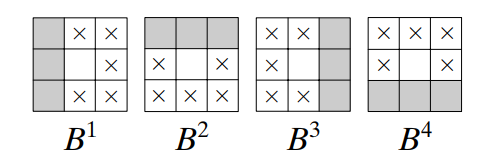
\includegraphics[width=0.4\linewidth]{fig/convex_hull_SE.png}
\end{figure}
\[X_k^i=(X_{k-1}\circledast B^i)\cup A\quad i=1,2,3,4\quad k=1,2,\ldots\]
其中$X_0^i=A$,当该过程收敛$X_k=X_{k-1}^i$时,令$D^i=X_k^i$,则$A$的凸壳为
\[C(A)=\bigcup_{i=1}^4 D^i\]
凸缺为凸包减去原集合
\item 细化
\[A\otimes B=A-(A\circledast B)=A\cap(A\circledast B)^C\]
\item 粗化
\[A\odot B=A\cup (A\circledast B)\]
\item 骨架
\[S(A)=\bigcup_{k=0}^K S_k(A)\]
其中
\[S_k(A)=(A\ominus kB)-(A\ominus kB)\circ B\]
\item 裁剪
\[\begin{aligned}
X_1&=A\otimes \{B\}\\
X_2&=\bigcup_{k=1}^8(X_1\circledast B^k)\\
X_3&=(X_2\oplus H)\cap A\\
X_4&=X_1\cup X_3
\end{aligned}\]
\end{itemize}

\subsection{灰度级形态学}
\begin{definition}[灰度级腐蚀与膨胀]
对非平坦结构元$b_N$的腐蚀
\[[f\ominus b](x,y)=\min_{(s,t)\in b}\{f(x+s,y+t)\}-b_N(s,t)\]
对非平坦结构元$b_N$的膨胀
\[[f\oplus b](x,y)=\max_{(s,t)\in b}\{f(x-s,y-t)\}+b_N(s,t)\]
\end{definition}

开操作与闭操作都有类似的定义及结论。

\begin{definition}[形态学梯度]
\[g=(f\oplus b)-(f\ominus b)\]
\end{definition}

\begin{definition}[顶帽与底帽变换]
顶帽(top-hat)变换
\[T_{hat}(f)=f-(f\circ b)\]
底帽(bottom-hat)变换
\[B_{hat}(f)=(f\bullet b)-f\]
\end{definition}

\begin{figure}[H]
\centering
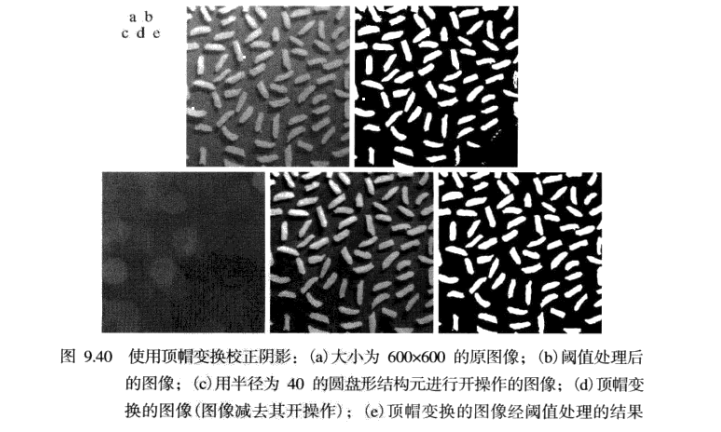
\includegraphics[width=0.8\linewidth]{fig/top-hat.png}
\end{figure}

粒度测定原理:以某一特定的尺度对含有相近尺度颗粒的图像区域进行\textbf{开操作},然后通过计算输
入图像和输出图像之间的差异可以对相近尺寸颗粒的相对数量进行测算。
\begin{figure}[H]
\centering
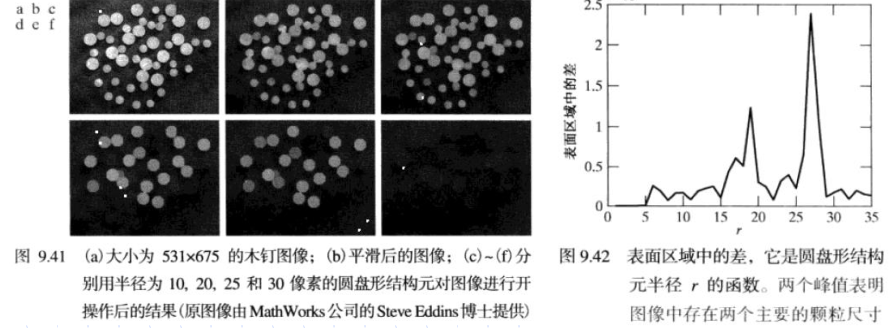
\includegraphics[width=\linewidth]{fig/granulometry.png}
\end{figure}

纹理分割:右边区域的圆点直径比左边大,目的是以纹理为基础找到区域的边界。
算法如下:
\begin{itemize}
\item [(a)] 取尺寸与小斑点大小的结构元素做闭运算(半径30)
\item [(b)] 取比大斑点间隙大的结构元素做开操作(半径60)
\item [(c)] 做二值化(使用全1的$3\times 3$结构元执行梯度画界)
\end{itemize}
\begin{figure}[H]
\centering
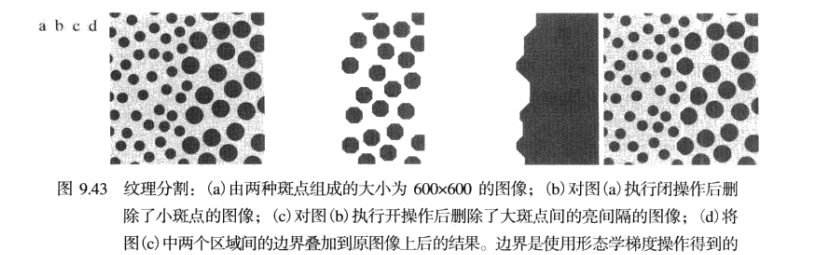
\includegraphics[width=\linewidth]{fig/texture_segment.png}
\end{figure}